Este filtro consiste b\'asicamente en dados un color y una distancia pasados como par\'ametros, procesa cada pixel de una im\'agen a color evaluando si el color del mismo se ''aleja'' m\'as de la distancia del par\'ametro, y si eso pasa, el p\'ixel se transforma a escala de grises, sino lo mantiene igual. Esto logra el efecto de resaltar un color en una im\'agen.

\subsubsection{Implementación en C}
Mediante dos ciclos anidados, se recorre la im\'agen por cada componente de color de cada pixel. Por cada pixel se levantan sus 3 colores RGB para calcular la distancia a los 3 colores RGB pasados por par\'ametro. Si el color de la im\'agen supera esa distancia, entonces en el p\'ixel que se est\'a procesando quedan sus 3 colores iguales unos con otros, logrando convertirse a blanco y negro. Si el color no supera la distancia, debe mantenerse tal cual, logrando as\'i ser resaltado.\\
Se define la distancia entre colores c\'omo:\\

\begin{center}
$distancia((r, g, b), (rc, gc, bc)) = \sqrt{(r - rc)^2 + (g - gc)^2 + (b - bc)^2}$
\end{center}

Para pasar a blanco y negro el p\'ixel, ponemos en cada canal de color (rgb), el mismo valor: $\frac{r + g + b}{3}$.

\subsubsection{Implementación en Assembler}
Haciendo uso de los registros \emph{XMM} por cada acceso a memoria se pueden traer 16 bytes con lo cual la cantidad de accesos a memoria decrementa 
considerablemente, haciendo que en comparaci\'on con el co\'odigo en C este sea mas optimo ya que el acceso a memoria es de las operaciones que mas 
consumen en cantidad de ciclos haciendo que disminuya la performance. Esto podr\'a apreciarse en la secc\'on de resultados.\newline
Al levantar los 16 bytes, lo primero que realizo es copiar estos 16 bytes en otros 2 registros \emph{XMM} para luego ordernarlos mediante la instrucc\'on
de Shuffle para que queden de la siguiente forma:

\begin{center}
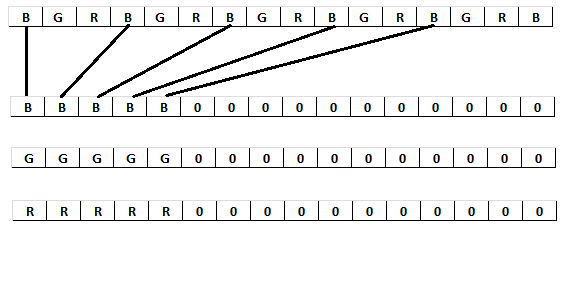
\includegraphics{imagenes/ImagenReorden.png}  
\end{center}

Luego le restamos a cada uno de los datos dentro de nuestros registros, un valor rc, bc o gc que es pasado por par\'matro, seg\'un se explica al
comienzo de esta secci\'on. Una considera\'on que vale la pena aclarar es que la resta es una diferencia absoluta. Este recaudo se tuvo que tomar dado 
que los bytes de la matriz son \emph{unsigned char} con lo cual si restabamos a un valor mas chico un valor mas grande esto pod\'ia confundirse y dejarnos
un valor que de ser una resta con sino ser\'ia v\'alido pero para nosotros no era util. Siendo esto, se toma compara el valor m\'as grande de cada dato
dentro del registro y el mas chico y se separan ambos en dos registros distintos. Luego se hace una resta del modo MAX - MIN dejando la resta sin signo
como quer\'iamos. A modo de ejemplo dejamos la siguiente imagen:

\begin{center}
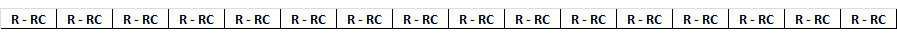
\includegraphics[width=16cm]{imagenes/resta.png} 
\end{center}

Una vez hecha la resta, se procede a convertir a float ya que las siguientes operaciones son multiplicaci\'on, suma y raiz cuadrada para la cual necesitamos
convertir nuestros datos a Float. La cuenta realizada por cada pixel es la siguiente:

\begin{center}
 $\sqrt{(r - rc)^2 + (g - gc)^2 + (b - bc)^2}$
\end{center}

Al final de toda la operaci\'on dejamos en 2 registros los 5 floats con cada una de estas operaciones en cada pixel. La siguiente imagen queda a forma de
entendimiento:

\begin{center}
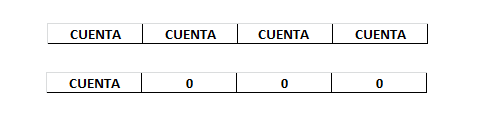
\includegraphics{imagenes/FinOperacion.png} 
\end{center}
 Un vez qu tenemos estos valores y luego de convertirlos a INT de tamaño Double word. Mediante el uso de la instrucci\'on PCMPGTD, comparamos que datos son
mayores y cuales son menores o iguales al valor pasado por parametro \emph{threshold} generando una mascara con valores 0xffffffff si el resultado de la 
operaci\'on dio \emph{true} y 0x0 en otro caso.\newline
Ya con esta m\'ascara generada, copiamos en 2 registros los valores originales de la matriz, y dejamos en uno los valores que queremos procesar usando la
instrucci\'on PAND y en otro los valores que queremos dejar como est\'an en el original usando PXOR de la m\'ascara y un PAND contra el registro. De esta
 manera negamos la m\'ascara y nos quedamos con los otros.\newline
Para terminar, procesamos los datos que debemos realizar la siguiente cuenta en para cada pixel:

\begin{center}
 $\frac{b + g + r}{3}$
\end{center}

Por \'ultimo solo le agregamos los resultados de los bits procesados al registro que tiene los datos originales y lo guardamos en la matriz de destino.

\subsubsection{Consideraci\'ones seg\'un optimizaciones}
\begin{itemize}
 \item Usando la herramienta \emph{objdump} desensamblamos el archivo .o de c\'odigo del filtro de Color. Al observar este c\'odigo, lo primero que notamos es
 que el compilador no us\'o instrucci\'ones de SIMD a pesar de que el procesador tenga esa caracteristica. Esto se debe a que al escribir en lenguaje C
no se puede hacer uso de estas operaciones a menos que usemos una librer\'ia aparte que haga uso de estas como puede ser \emph{libSIMDx86}.\newline
En cuanto a como se manipulas las variables locales, Se respetan las convenciones de pushear registros como r15 - r12 y rbx. Pero en casi todo el c\'odigo
se hace uso de las variables por parametros y se usa mucho la pila moviendo el registro rbp para recorrerla.\newline
\item Existen algunas optimizaciones que se pueden realizar a la hora de compilar el c\'odigo en C. Estas son -O1, -O2 o -O3, las cuales, siendo agregadas
como flags a la hora de compilar, mi c\'odigo ensamblado queda mucho m\'as \'optimo. En particular el flag -O1 hace que el tamaño del c\'odigo ensamblado
sea mucho menor que el c\'odigo ensablado sin optimizaci\'on. En particular al mirar el objdump de c\'odigo con -O1 se pudo apreciar que el c\'odigo era
mucho menor en cantidad de lineas y que la cantidad de registros pusheados a la pila fue mayor.\newline
El flag -O2 hace todas las optimizaciones que pueda en el c\'odigo que no est\'en involucradas con optimizaciones de espacio-tiempo. Y por \'ultimo el flags
-O3 abre todas las opmitizaciones de -O2 mas algunas extras con el fin de hacer aun m\'as optimo el c\'odigo.\footnote{Para mas informaci\'on revisar el
http://gcc.gnu.org/onlinedocs/gcc/Optimize-Options.html}\newline
\item Haciendo uso de las optimizaciones mencionadas anteriormente, se realizaron experimentos de performance usando el c\'odigo en ASM, en C y en C 
compilado con optimizacion -O1, -O2 y -O3. El siguiente gr\'afico muestra como el c\'odigo en C optimizado y el ASM son casi id\'enticos.

\begin{center}
 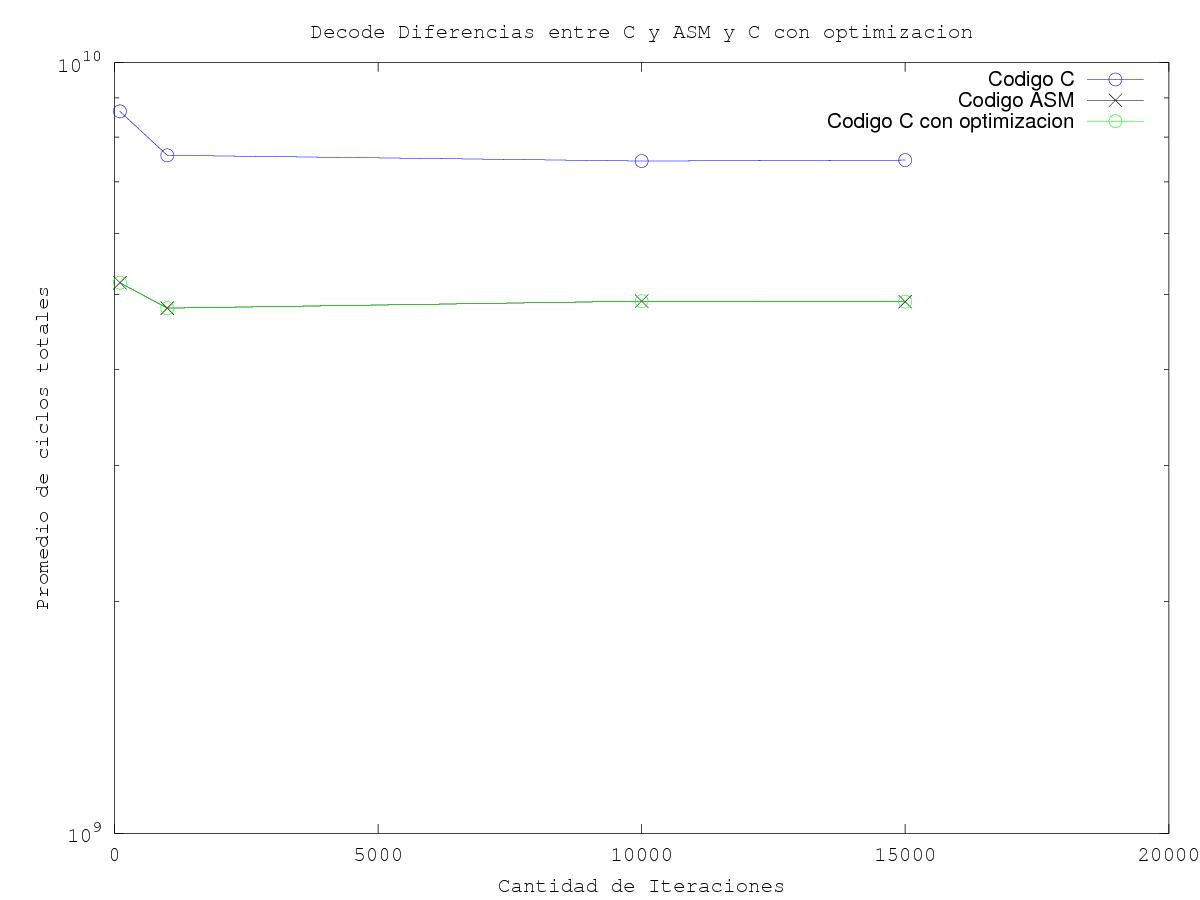
\includegraphics[scale=0.5]{imagenes/optimizacionC.jpg}
\end{center}

Esta medici\'on fue realizada cambiando la cantidad de iteraciones y midiendo cuantos ticks de procesador consume procesar el video completo. El 
problema de realizar las mediciones de esta manera es que el procesador switchea entre distintos procesos todo el tiempo haciendo que mi contador aumente
 al ejecutar procesos que no pertenecen a mi funci\'on y se cuenta en intervalos muy grandes provocando que la probabilidad de contar ticks de procesos
 exteriores sea mayor. Es por esta raz\'on que nuestra medici\'on no es lo suficientemente precisa. Una forma de hacerla mas precisa ser\'ia evaluando un
promedio de la cantidad de Ticks que consume por cada frame de cada iteraci\'on. Pero al trabajar en ordenes tan grandes deber\'iamos procesar demasiada
 informaci\'on que no viene al caso de lo que se queire mostrar.\newline

\end{itemize}

\subsubsection{Loop unrolling}
Loop unrolling, o desenrollado de ciclo en español, es una t\'ecnica de optimizaci\'on que consiste en transformar un bucle para mejorar la velocidad de ejecuci\'on de un programa. La transformaci\'on puede llevarse a cabo por el programador o por un compilador de optimizaci\'on.\\
La t\'ecnica se basa en eliminar las instrucciones que controlan el bucle, por ejemplo, reduciendo la cantidad de iteraciones que tiene que pasar un ciclo, evitando comparar menos veces si se termin\'o de iterar o no.\\
Por ejemplo:

\begin{center}
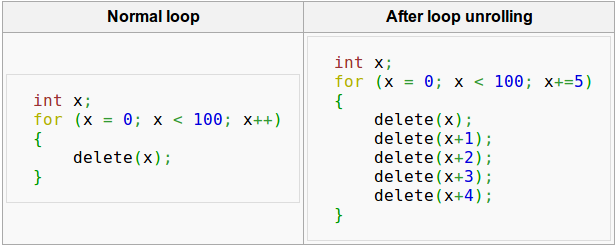
\includegraphics[scale=0.5]{imagenes/loopunrolling_ejemplo.png}
\end{center}

Como podemos ver, el ciclo desenrollado recorre menos veces, por lo tanto hace menos comparaciones. Pero corre con la gran desventaja de que se genera mucho m\'as c\'odigo.\\
Una forma de aplicarlo a nuestro filtro de color en C es procesar m\'as cantidad de p\'ixels. En nuestro filtro C com\'un procesamos de a 1 p\'ixel. Probamos procesar de a 2 p\'ixels, donde el procesamiento de columnas, o de ancho de la im\'agen se reduce a la mitad. Sin embargo, midiendo velocidades, no detectamos grandes diferencias, ya que esa optimizaci\'on no es muy significativa o el compilador de C tal vez haga esta optimizaci\'on.\\
Luego probamos optimizando m\'as, procesando de a 6 p\'ixels en el C y ahorrando ciertos accesos a memoria. Los resultados fueron m\'as notorios:

\begin{center}
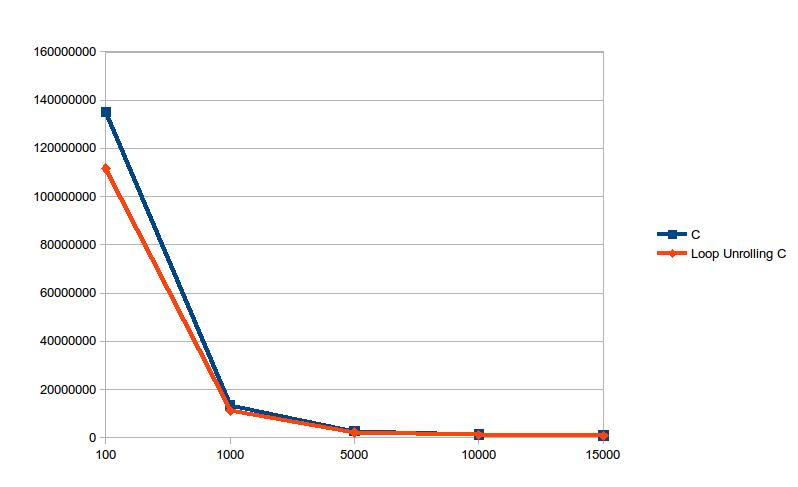
\includegraphics[scale=0.5]{imagenes/loopunrolling_c.jpg}
\end{center}

El eje x son la cantidad de iteraciones y el eje y es el tiempo que tard\'o para cierta cantidad de iteraciones.\\
En velocidad vemos la mejora del loop unrolling, pero en c\'odigo incrementa considerablemente.\\\\

En cuanto al c\'odigo ASM resulta m\'as complejo hacer esta optimizaci\'on ya que procesamos de a 5 p\'ixels, lo que entra en un registro XMM.\\
Lo que probamos fue copiar ese procesamiento de 5 p\'ixels, para procesar id\'enticamente la misma cantidad dentro del ciclo. Es decir que dentro de un mismo bucle procesamos 5 p\'ixels, y luego otros 5, procesando de a 10 en un mismo bucle. De esta manera nos ahorramos que se ejecuten las dos instrucciones de control del ciclo la mitad de las veces:\\

.ciclo:\\
CMP rcx, 0\\
JLE .fin\\

Midiendo tiempos de ejecuci\'on nos damos cuenta que no hay grandes diferencias con el ASM implementado sin aplicar esta t\'ecnica. Al parecer ahorrar 2 instrucciones b\'asicas de assembler para el tamaño de im\'agen que probamos (960 x 540), no es significativo.\\
Vale aclarar que la cantidad de pixels en ancho o en alto debe ser multiplo de 10, sino habr\'ia que tener ciertas consideraciones.


